\section{Structure through equivalence}
%%%%%%%%%%%%%%%%%%%%%%%%%%%%%%%%%%%%%%%%%%%%%%%%%%%%%%%%%
\subsection{Motivation}

We now have \draftnote{blue}{awjdean}{Improve this - include stuff like the set $\mathcal{T}$.}
\begin{enumerate}
	\item an infinite set $D$ of transformations, which are walks in the multidigraph $\mathscr{W}=(W, \hat{D}, s, t)$;

	\item an infinite set $D_{A}$ of action transformations, which are walks in the multidigraph $\mathscr{W}_{A}=(W, \hat{D}_{A}, s, t)$;

	\item an infinite, but less dense, set $\hat{A}^{\ast}$ of actions;

	\item a labelling map $l: D_{A} \to \hat{A}^{\ast}$ that allows us to construct an infinite number of functions $f_{a}$ that describe the effect of the actions in $\hat{A}^{\ast}$; and

	\item a free monoid algebra $(\hat{A}^{\ast}, \; \circ)$.
\end{enumerate}


Our basic algebra of actions $(\hat{A}^{\ast}, \; \circ)$ is a (countably infinite) free monoid; this is the same for any world.
However, we expect that there must be more structure we can tease out of our $(\hat{A}^{\ast}, \; \circ)$ since it appears that different worlds have different transformation structures.
But how do we produce those structures from $(\hat{A}^{\ast}, \; \circ)$ ?
If we want to form other recognisable algebraic structures (e.g., groups, semigroups etc...), we need some way of saying collections of transformations (i.e., the actions that are elements of $\hat{A}^{\ast}$) are the same in some way, otherwise, there is no way to satisfy the requirements of these algebras (\textit{e.g.}, for the inverse property we need an element $a'$ in $\hat{A}^{\ast}$ for each $a \in \hat{A}^{\ast}$ such that $a' \circ a = \varepsilon$ and $a \circ a' = \varepsilon$).

To solve this issue and to enforce the structure of the world on the algebra $(\hat{A}^{\ast}, \; \circ)$, we will define an equivalence relation $\sim$ on the elements of $\hat{A}^{\ast}$.
This equivalence relation will enforce aspects of the structure of the world onto the free monoid $(\hat{A}^{\ast}, \; \circ)$ to give us a new algebra $(\hat{A}^{\ast}/\sim, \; \circ_{\sim})$ \draftnote{blue}{awjdean}{Do we actually need congruences?}, where it is now possible to satisfy properties like the inverse condition.

Additionally, considering the learning problem of the agent, as it stands, our agent would need to learn an infinite number of transformations (the elements of $D$) each of which is specific to individual world states or the effect of an infinite number of actions to learn the structure of the world (the structure of $(\hat{A}^{\ast}, \circ, \ast)$).
The structure of the new algebra $(\hat{A}^{\ast}/\sim, \; \circ_{\sim})$ should be easier for an agent to learn than learning every element in an infinite set.
We also believe agents can gain a better understanding of the structure of the world though learning the structure of the algebras we will construct using equivalence relations \draftnote{blue}{awjdean}{
	We actually think this is what agent's do when they learn the structure of the world
}.

\footnote{
	When we define an equivalence $\sim$ on $\hat{A}^{\ast}$ to get the set $\hat{A}^{\ast}/\sim$, we can think of our set $\hat{A}^{\ast}$ `folding over' on itself to make elements of $\hat{A}^{\ast}$ that are equivalent stick together.
}



\whendraft{
	\draftnote{red}{DIVIDER}{}
	\draftnote{blue}{awjdean}{Do something with this - something about how extracting the global algebra provides generalisation potential.
	}
	We can also describe the effect $\ast: \hat{A}^{\ast} \times W \to W$ of the actions of the agent on the world $\mathscr{W} = (W, \hat{D}, s, t)$ as the action of the (global) algebra $(\hat{A}^{\ast}, \circ)$ on the set $W$.
	If such a global algebra exists, then it is possible for our agent to learn the structure of $(\hat{A}^{\ast}, \circ)$ and so understand the transformation structure of its actions without considering its current world state; this could have powerful generalisation capabilities.
	\draftnote{blue}{awjdean}{
		I currently think that a global algebra does always exist, but that sometimes it's horrible and doesn't really abstract away the effect of the actions from the world states since it requires a map that connects to the world states to tell the algebra on which world states things are and aren't defined.
	}
	\draftnote{red}{DIVIDER}{}
}

%%%%%%%%%%%%%%%%%%%%%%%%%%%%%%%%%%%%%%%%%%%%%%%%%%%%%%%%%
\subsection{An equivalence relation: $\sim$}

We define an equivalence relation on the elements of $\hat{A}^{\ast}$ that says two actions are equivalent (our sense of the actions being the same) if they lead to the same end world state when performed in any initial world state. \draftnote{blue}{awjdean}{Footnote about how this was inspired by \autocite{caselles2020sensory} is our mathematical interpretation of equality in \autocite{Higgins2018}.}

\begin{definition}[Equivalence of actions under $\sim$]
	Given two actions $a, a' \in \hat{A}^{\ast}$,
	\begin{equation}
		a \sim a' \iff a \ast w = a' \ast w \quad \text{ for all $w \in W$}
	\end{equation}
\end{definition}

\draftnote{blue}{awjdean}{Footnote about this being true for actions leading to the undefined state (and why).}

\begin{proposition}
	$\sim$ is an equivalence relation on $\hat{A}^{\ast}$.
\end{proposition}
\begin{proof}
	\draftnote{blue}{awjdean}{Check/improve this.}
	\textbf{Reflexive.}
	If $a \sim a'$ then $a \ast w = a' \ast w$ for all $w \in W$, and so $a \sim a$.

	\textbf{Transitive.}
	If $a \sim a'$ and $a' \sim a''$, then $a \ast w = a' \ast w$ for all $w \in W$ and $a' \ast w = a'' \ast w$ for all $w \in W$.
	Therefore, $a \ast w = a'' \ast w$ for all $w \in W$ and so $a \sim a''$.

	\textbf{Symmetric.}
	If $a \sim a'$, then $a \ast w = a' \ast w$ for all $w \in W$.
	Therefore $a' \ast w = a \ast w$ for all $w \in W$, and so $a' \sim a$.
\end{proof}

We define the canonical projection map $\pi_{A}: \hat{A}^{\ast} \to \hat{A}^{\ast}/\sim$ that sends actions in $\hat{A}^{\ast}$ to their equivalence classes under $\sim$ in the quotient set $\hat{A}^{\ast}/\sim$:
\begin{equation}
	\pi_{A}: \hat{A}^{\ast} \to \hat{A}^{\ast}/\sim \text{ where } \pi_{A}(a) = [a]_{\sim}
\end{equation}
This projection map $\pi_{A}$ effectively collapses actions with identical effects into a single representative.
The equivalent classes $[a]_{\sim}$, where $[a]_{\sim}$ denotes the equivalence class of $a$ due to $\sim$, are
\begin{equation}
	[a]_{\sim} = \{ a' \in \hat{A}^{\ast} \mid a' \sim a \}
\end{equation}

Sometimes we will drop the $[a]_{\sim}$ in favour of $a \in \hat{A}^{\ast}/\sim$ for ease.

\paragraph{Composition of actions}
We define the composition of elements in $\hat{A}^{\ast}/\sim$ using our action composition operator $\circ$ as
\begin{equation}
	\begin{aligned}
		 & \circ_{\sim}: (\hat{A}^{\ast}/\sim) \times (\hat{A}^{\ast}/\sim) \to (\hat{A}^{\ast}/\sim) \quad \text{such that} \\
		 & [a']_{\sim} \circ_{\sim} [a]_{\sim} = [a' \circ a]_{\sim} \quad \text{for $a,a' \in \hat{A}^{\ast}$}
	\end{aligned}
\end{equation}


We need to show that the operation $\circ_{\sim}$ on the equivariance classes does not depend on the representative element chosen for those classes; this means we can consistently use any element of an equivalence class as a representative of that class.

\begin{proposition}\label{prp:circ_sim_well_defined}
	$\circ_{\sim}$ is well-defined on $\hat{A}^{\ast}/\sim$.
\end{proposition}
\begin{proof}
	\begin{enumerate}
		\item \textbf{Problem.}
		      For $\circ_{\sim}$ to be well-defined on $\hat{A}^{*}/\sim$, we need that\footnote{
			      \textbf{Well-definedness requirement.}
			      An operation on a quotient set
			      \begin{equation}
				      (\hat{A}^{*}/\sim) \times (\hat{A}^{*}/\sim) \to \hat{A}^{*}/\sim
			      \end{equation}
			      is \emph{well-defined} if take different representatives of the same equivalence classes doesn't change the resulting equivalence class.
			      Mathematically,
			      \begin{equation}
				      \begin{aligned}
					               & [a]_{\sim} = [b]_{\sim} \; \text{and} \; [a']_{\sim} = [b']_{\sim} \\
					      \implies & [a' \circ a]_{\sim} = [b' \circ b]_{\sim}
				      \end{aligned}
			      \end{equation}
		      }
		      \begin{equation}
			      \begin{aligned}
				       & \text{If $[a]_{\sim} = [b]_{\sim}$ and $[a']_{\sim} = [b']_{\sim}$, then} \\
				       & [a' \circ a]_{\sim} = [b' \circ b]_{\sim}
			      \end{aligned}
		      \end{equation}

		\item \textbf{Initial assumptions.}
		      For $a, b, a', b' \in \hat{A}^{\ast}$:
		      \begin{itemize}
			      \item $a \sim b$ means:
			            \begin{equation}
				            a \ast w = b \ast w \quad \text{for all } w\in W
			            \end{equation}
			      \item $a' \sim b'$ means:
			            \begin{equation}
				            a' \ast w = b' \ast w \quad \text{for all } w\in W
			            \end{equation}
		      \end{itemize}

		\item \textbf{Goal.}
		      We want to show $[a' \circ a]_{\sim} = [b' \circ b]_{\sim}$.
		      \begin{align}
			                    & [a' \circ a]_{\sim} = [b' \circ b]_{\sim}                               \\
			      \Rightarrow{} & (a' \circ a) \sim (b' \circ b)                                          \\
			      \Rightarrow{} & (a' \circ a) \ast w = (b' \circ b) \ast w \quad \text{for all } w \in W
		      \end{align}

		\item \textbf{Proof.}
		      We have:
		      \begin{equation}
			      (a' \circ a) \ast w = a' \ast (a \ast w).
		      \end{equation}
		      Similarly, we have:
		      \begin{equation}
			      (b' \circ b) \ast w = b' \ast (b \ast w).
		      \end{equation}
		      Since $a \sim b$, we have $a \ast w = b \ast w$ for all $w \in W$.
		      Therefore,
		      \begin{align}
			          & (a' \circ a) \ast w \\
			      ={} & a' \ast (a \ast w)  \\
			      ={} & a' \ast (b \ast w)
		      \end{align}
		      Since $a' \sim b'$, we have $a' \ast w = b' \ast w$ for all $w \in W$.
		      Therefore,
		      \begin{align}
			          & (a' \circ a) \ast w  \\
			      ={} & b' \ast (b \ast w)   \\
			      ={} & (b' \circ b) \ast w.
		      \end{align}


		\item \textbf{Conclusion.}
		      We have shown that $(a' \circ a) \ast w = (b' \circ b) \ast w$, and therefore $(a' \circ a) \sim (b' \circ b)$, and hence $\circ_{\sim}$ is well-defined on $\hat{A}^{\ast}/\sim$.
	\end{enumerate}
\end{proof}

\begin{proposition}\label{prp:circ_sim_closed}
	$\circ_{\sim}: (\hat{A}^{\ast}/\sim) \times (\hat{A}^{\ast}/\sim) \to \hat{A}^{\ast}/\sim$ is closed.
\end{proposition}
\begin{proof}
	$\circ_{\sim}$ is closed $\circ_{\sim}$ is the images under $\pi_{A}$ of the concatenation operation $\circ$ in $\hat{A}^{\ast}$, and all elements of $\hat{A}^{\ast}$ have equivalence classes in $\hat{A}^{\ast}/\sim$.
\end{proof}


Now we have proved that $\circ_{\sim}$ is well-defined on $\hat{A}^{\ast}/\sim$ we denote $\circ_{\sim}$ by $\circ$ when it is obvious what we mean\footnote{$\circ_{\sim}$ can be thought of as the composition operator $\circ$ after it has been pulled through the map $\pi_{A}$.}.

\paragraph{Effect of equivalent actions on world states.}
We define the effect of an element of  $\hat{A}^{\ast}/\sim$ on world states as
\begin{equation}
	\begin{aligned}
		 & \ast_{\sim}: (\hat{A}^{\ast}/\sim) \times W \to W \quad \text{such that} \\
		 & [a]_{\sim} \ast_{\sim} w = a \ast w
	\end{aligned}
\end{equation}

\begin{proposition}
	$\ast_{\sim}$ is well-defined on $\hat{A}^{\ast}/\sim$.
\end{proposition}
\begin{proof}
	To prove that $\ast_{\sim}$ is well-defined, we need to show that if two actions $a, b \in \hat{A}^{\ast}$ are equivalent (i.e., $a \sim b$), then they have the same effect on any world state $w$.

	\begin{enumerate}
		\item \textbf{Initial assumption.}
		      Let $a \sim b$.
		      By definition of the equivalence relation $\sim$, we have
		      \begin{align}
			       & a \ast w = b \ast w \quad \text{for all } w \in W
		      \end{align}

		\item \textbf{Definition of $\ast_{\sim}$.}
		      By definition, the effect of $[a]_{\sim}$ on a world $w$ is given by
		      \begin{equation}
			      [a]_{\sim} \ast_{\sim} w = a \ast w
		      \end{equation}
		      Similarly, the effect of $[b]_{\sim}$ on a world $w$ is given by
		      \begin{equation}
			      [b]_{\sim} \ast_{\sim} w = b \ast w
		      \end{equation}

		\item \textbf{Goal.}
		      We want to prove that
		      \begin{equation}
			      [a]_{\sim} \ast_{\sim} w = [b]_{\sim} \ast_{\sim} w
		      \end{equation}
		      Which is equivalent to proving that:
		      \begin{equation}
			      a \ast w = b \ast w.
		      \end{equation}

		\item \textbf{Proof.}
		      Since $a \sim b$, we have $a \ast w = b \ast w$ by the definition of $\sim$.

		\item \textbf{Conclusion.}
		      We have shown that $a \ast w = b \ast w$.
		      This implies that
		      \begin{equation}
			      [a]_{\sim} \ast_{\sim} w = [b]_{\sim} \ast_{\sim} w
		      \end{equation}
		      Therefore, $\ast_{\sim}$ is well-defined on $\hat{A}^{\ast}/\sim$.
	\end{enumerate}
\end{proof}

Now we have proved that $\ast_{\sim}$ is well-defined on $\hat{A}^{\ast}/\sim$ we denote $\ast_{\sim}$ by $\ast$ where it is obvious what we mean\footnote{$\ast_{\sim}$ can be thought of as the composition operator $\ast$ after it has been pulled through the map $\pi_{A}$.}.

%%%%%%%%%%%%%%%%%%%%%%%%%%%%%%%%%%%%%%%%%%%%%%%
\subsection{New structures from $\sim$}

Applying our projection map $\pi_{A}$ to the structures $(\hat{A}^{\ast}, \circ)$, $(\hat{A}^{\ast}, \circ, \ast)$, and $\mathcal{T}_{\hat{A}^{\ast}}$ gives us these new structures:
\begin{align}
	 & \pi_{A}(\text{ }(\hat{A}^{\ast}, \circ)\text{ }) = (\hat{A}^{\ast}/\sim, \circ_{\sim})                    \\
	 & \pi_{A}(\text{ }(\hat{A}^{\ast}, \circ, \ast)\text{ }) = (\hat{A}^{\ast}/\sim, \circ_{\sim}, \ast_{\sim}) \\
	 & \pi_{A}(\text{ }\mathcal{T}_{\hat{A}^{\ast}}\text{ }) = \mathcal{T}_{\hat{A}^{\ast}/\sim}
\end{align}
\footnote{Technically $\pi_{A}(\text{ }\mathcal{T}_{\hat{A}^{\ast}}\text{ }) = \mathcal{T}_{\hat{A}^{\ast}/\sim}$ implies that the functions $f_{a}$ induced by individual actions $a \in \hat{A}^{\ast}$ correspond exactly to the functions $f_{[a]_{\sim}}$ induced by the equivalence classes in $\hat{A}^{\ast}/\sim$.
We will prove this soon.}


\subsection{$(\hat{A}^{\ast}/\sim, \circ_{\sim})$.}
Applying the equivalence relation $\sim$ using the projection $\pi_{A}$ to the free monoid $(\hat{A}^{\ast}, \circ)$ gives the quotient monoid $(\hat{A}^{\ast}/\sim, \circ_{\sim})$\footnote{
	$(\hat{A}^{\ast}/\sim, \circ_{\sim})$ is the homomorphic image of $(\hat{A}^{\ast}, \circ)$ through the projection $\pi_{A}$.
}, whose elements are the equivalence classes $[a]_{\sim}$ for all $a \in \hat{A}^{\ast}$.

\begin{propositionE}\label{prp:circ_sim_associative}
	$\circ_{\sim}$ is associative on $\hat{A}^{\ast}/\sim$.
\end{propositionE}
\begin{proofE}
	Associativity of $\circ_{\sim}$ comes from the associativity of $\circ$.
	\begin{align}
		     & ([a'']_{\sim} \circ_{\sim} [a']_{\sim}) \circ_{\sim} [a]_{\sim} \\
		= \; & [a'' \circ a']_{\sim} \circ_{\sim} [a]_{\sim}                   \\
		= \; & [ (a'' \circ a') \circ a ]_{\sim}                               \\
		= \; & [ a'' \circ (a' \circ a) ]_{\sim}                               \\
		= \; & [a'']_{\sim} \circ_{\sim} [a' \circ a]_{\sim}                   \\
		= \; & [a'']_{\sim} \circ_{\sim} ([a']_{\sim} \circ_{\sim} [a]_{\sim})
	\end{align}
\end{proofE}


\begin{proposition}\label{prp:A_sim_identity}
	$[\varepsilon]_{\sim}$ is the identity element of $(\hat{A}^{\ast}/\sim, \; \circ_{\sim})$.
\end{proposition}
\begin{proof}
	For any $[a]_{\sim} \in \hat{A}^{\ast}/\sim$, we have
	\begin{align}
		 & [\varepsilon]_{\sim} \circ_{\sim} [a]_{\sim} = [\varepsilon \circ a]_{\sim} = [a]_{\sim}
		 & [a]_{\sim} \circ_{\sim} [\varepsilon]_{\sim} = [a \circ \varepsilon]_{\sim} = [a]_{\sim}
	\end{align}
	Therefore, $[\varepsilon]_{\sim}$, where $\varepsilon$ is the empty action, acts as the identity.
\end{proof}


\begin{proposition}\label{prp:A_sim_is_monoid}
	$(\hat{A}^{\ast}/\sim, \circ_{\sim})$ is a monoid.
\end{proposition}
\begin{proof}
	\begin{enumerate}
		\item \textbf{Closure and well-definedness.}
		      We need to show that the operation $\circ_{\sim}$ is well-defined and closed on $\hat{A}^{\ast}/\sim$.
		      $\circ_{\sim}$ is well-defined on $\hat{A}^{\ast}/\sim$ from proposition \ref{prp:circ_sim_well_defined} and closed from proposition \ref{prp:circ_sim_closed}.

		\item \textbf{Associativity.}
		      Given by proposition \ref{prp:circ_sim_associative}.

		\item \textbf{Identity Element.}
		      Given by proposition \ref{prp:A_sim_identity}.

		\item \textbf{Conclusion.}
		      The structure $(\hat{A}^{\ast}/\sim, \circ_{\sim})$ is a monoid.
	\end{enumerate}
\end{proof}

Now can now show that $\pi_{A}$ preserves the monoid structure of $(\hat{A}^{\ast}, \circ)$, and so $\pi_{A}$ is a monoid homomorphism.
\begin{proposition}
	$\pi_{A}$ is a monoid homomorphism from $(\hat{A}^{\ast}, \circ)$ to $(\hat{A}^{\ast}/\sim, \circ_{\sim})$.
\end{proposition}
\begin{proof}
	\begin{enumerate}
		\item \textbf{Preservation of the Operation.}
		      For any $a, a' \in \hat{A}^{\ast}$, the projection $\pi_{A}$ satisfies:
		      \begin{align}
			      \pi_{A}(a \circ a') & = [a \circ a']_{\sim}                 \\
			                          & = [a]_{\sim} \circ_{\sim} [a']_{\sim} \\
			                          & = \pi_{A}(a) \circ_{\sim} \pi_{A}(a')
		      \end{align}
		      Thus:
		      \begin{equation}
			      \pi_{A}(a \circ a') = \pi_{A}(a) \circ_{\sim} \pi_{A}(a').
		      \end{equation}

		\item \textbf{Preservation of the Identity Element.}
		      The identity element in $(\hat{A}^{\ast}, \circ)$ is $\varepsilon$, and the identity element in $(\hat{A}^{\ast}/\sim, \circ_{\sim})$ is $[\varepsilon]_{\sim}$.
		      The projection satisfies:
		      \begin{equation}
			      \pi_{A}(\varepsilon) = [\varepsilon]_{\sim}.
		      \end{equation}

		\item \textbf{Conclusion.}
		      The projection $\pi_{A}$ is a monoid homomorphism.
	\end{enumerate}
\end{proof}

If the number of distinct effects on $W$ is finite, then $(\hat{A}^{\ast}/\sim, \circ_{\sim})$ will have a finite number of elements.

%%%%%%%%%%%%%%%%%%%%%%%%%%%%%%%%%%%%%%%%%%%
\subsection{$(\hat{A}^{\ast}/\sim, \circ_{\sim}, \ast_{\sim})$.}

\begin{proposition}
	$(\hat{A}^{\ast}/\sim, \circ_{\sim}, \ast_{\sim})$ is a monoid action of $(\hat{A}^{\ast}/\sim, \circ_{\sim})$ on the set $W$.
\end{proposition}

\begin{proof}
	\begin{enumerate}
		\item \textbf{Compatibility.}
		      The action effect operator $\ast_{\sim}$ is compatible with the composition operator $\circ_{\sim}$ since:
		      \begin{equation}
			      ([a']_{\sim} \circ_{\sim} [a]_{\sim}) \ast_{\sim} w = [a']_{\sim} \ast_{\sim} ([a]_{\sim} \ast_{\sim} w) \quad \text{for all } [a]_{\sim}, [a']_{\sim} \in \hat{A}^{\ast}/\sim, \, w \in W.
		      \end{equation}

		      \textit{Proof:} By the definitions of $\circ_{\sim}$ and $\ast_{\sim}$, we have:
		      \begin{align}
			      ([a']_{\sim} \circ_{\sim} [a]_{\sim}) \ast_{\sim} w & = [a' \circ a]_{\sim} \ast_{\sim} w                   \\
			                                                          & = (a' \circ a) \ast w                                 \\
			                                                          & = a' \ast (a \ast w)                                  \\
			                                                          & = [a']_{\sim} \ast_{\sim} ([a]_{\sim} \ast_{\sim} w).
		      \end{align}
		      Therefore, the compatibility condition holds.

		\item \textbf{Identity action.}
		      The identity element $[\varepsilon]_{\sim}$ acts as the identity on $W$:
		      \begin{equation}
			      [\varepsilon]_{\sim} \ast_{\sim} w = w \quad \text{for all } w \in W.
		      \end{equation}

		      \textit{Proof:} Using the definition of $\ast_{\sim}$ and knowing that $\varepsilon$ is the empty action sequence, we get:
		      \begin{align}
			      [\varepsilon]_{\sim} \ast_{\sim} w & = \varepsilon \ast w \\
			                                      & = w.
		      \end{align}
		      Thus, $[\varepsilon]_{\sim}$ acts as the identity on $W$.

		\item \textbf{Conclusion.}
		      $(\hat{A}^{\ast}/\sim, \circ_{\sim}, \ast_{\sim})$ is a monoid action on the set $W$.
	\end{enumerate}
\end{proof}


%%%%%%%%%%%%%%%%%%%%%%%%%%%%%%%%%%%%%%%%%%%%%%%%%%
\subsection{$\mathcal{T}_{\hat{A}^{\ast}/\sim}$}

To explore the effect of applying the equivalence relation $\sim$ to the functions $f_{a} \in \mathcal{T}_{\hat{A}^{\ast}}$, we must first find the equivalent to applying $\sim$ on the functions $f_{a}$.

\begin{proposition}\label{prp:equivalence_equivalence_on_functions}
	$a \sim a' \iff f_{a}(w) = f_{a'}(w)$ for all $w \in W$.
\end{proposition}
\begin{proof}
	\begin{enumerate}
		\item \textbf{$a \sim a' \implies f_{a}(w) = f_{a'}(w)$ for all $w \in W$.}
		      Let $a \sim a'$. By the definition of $\sim$, this means:
		      \begin{equation}
			      a \ast w = a' \ast w \quad \text{for all } w \in W.
		      \end{equation}
		      The functions $f_{a}$ and $f_{a'}$ are defined as:
		      \begin{equation}
			      f_{a}(w) = a \ast w, \quad f_{a'}(w) = a' \ast w.
		      \end{equation}
		      From the assumption $a \ast w = a' \ast w$, we have:
		      \begin{equation}
			      f_{a}(w) = f_{a'}(w) \quad \text{for all } w \in W.
		      \end{equation}
		      Therefore, the functions $f_{a}$ and $f_{a'}$ are identical:
		      \begin{equation}
			      f_{a} = f_{a'}.
		      \end{equation}

		\item \textbf{$f_{a}(w) = f_{a'}(w)$ for all $w \in W$ $\implies$ $a \sim a'$.}
		      The functions $f_{a}$ and $f_{a'}$ are defined as:
		      \begin{equation}
			      f_{a}(w) = a \ast w, \quad f_{a'}(w) = a' \ast w.
		      \end{equation}
		      Since $f_{a}(w) = f_{a'}(w)$, it follows that:
		      \begin{equation}
			      a \ast w = a' \ast w \quad \text{for all } w \in W.
		      \end{equation}
		      By the definition of $\sim$, we conclude that:
		      \begin{equation}
			      a \sim a'
		      \end{equation}

		\item \textbf{Conclusion.}
		      Combining both directions, we have:
		      \begin{equation}
			      a \sim a' \iff f_{a}(w) = f_{a'}(w) \quad \text{for all } w \in W.
		      \end{equation}
	\end{enumerate}
\end{proof}

\draftnote{blue}{awjdean}{Does potential redundancy mean that $\{ f_{a} \mid a \in \hat{A}^{\ast} \}$ does not necessarily form a monoid ?}

As before with $\ast$, we can curry the action $\ast_{\sim}: (\hat{A}^{\ast}/\sim) \times W \to W$ to give a set of functions $f_{[a]_{\sim}}$.
We denote this set by $\mathcal{T}_{\hat{A}^{\ast}/\sim}$:
\begin{equation}
	\begin{aligned}
		 & \mathcal{T}_{\hat{A}^{\ast}/\sim} = \{ f_{[a]_{\sim}} \mid a \in \hat{A}^{\ast} \} \quad \text{where} \\
		 & f_{[a]_{\sim}}(w) = [a]_{\sim} \ast w = a \ast w \quad \text{for $a \in \hat{A}^{\ast}$}
	\end{aligned}
\end{equation}

The set $\mathcal{T}_{\hat{A}^{\ast}/\sim}$ is the set $\mathcal{T}_{\hat{A}^{\ast}}$ but with identical functions in $\mathcal{T}_{\hat{A}^{\ast}}$ now collapsed into a single representative in $\mathcal{T}_{\hat{A}^{\ast}/\sim}$.

\begin{proposition}
	$\mathcal{T}_{\hat{A}^{\ast}/\sim}$ is a monoid.
\end{proposition}
\begin{proof}
	The proof is trivial: $\mathcal{T}_{\hat{A}^{\ast}}$ is a monoid from proposition \ref{prp:T_is_monoid}.
	From proposition \ref{prp:equivalence_equivalence_on_functions}, the application of $\sim$ just means that functions where $f_{a}=f_{a'}$ are represented by a single function $f_{[a]_{\sim}}$ in $\mathcal{T}_{\hat{A}^{\ast}/\sim}$, which does not affect the properties of a monoid.
\end{proof}

Similarly to what we did with $\phi: \hat{A}^{\ast} \to \mathcal{T}_{\hat{A}^{\ast}}$, we define a map
\begin{equation}
	\begin{aligned}
		 & \Phi : \hat{A}^{\ast}/\sim \to \text{End}(W) \quad \text{where} \\
		 & \Phi([a]_{\sim}) = f_{[a]_{\sim}}
	\end{aligned}
\end{equation}
\footnote{$\text{End}(W)$ is the set of functions from $W$ to itself.
	Functions from a set to itself are called \emph{endomorphisms}.}

\begin{proposition}
	$\Phi$ is an injective homomorphism. \draftnote{blue}{awjdean}{Put $[]_{\sim}$'s in.}
\end{proposition}
\begin{proof}
	\begin{enumerate}
		To prove that $\Phi$ is an injective homomorphism we need to show that $\Phi$ is injective and a homomorphism.
		\item \textbf{Homomorphism.}
		      \begin{enumerate}
			      \item \textbf{Goal.}
			            We want
			            \begin{equation}
				            \Phi([a']_\sim \circ_\sim [a]_\sim) = \Phi([a']_\sim) \circ \Phi([a]_\sim) \quad \textit{for all $[a]_\sim, [a']_\sim \in \hat{A}^{\ast} / \sim$}
			            \end{equation}
			      \item \textbf{Proof.}
			            \begin{itemize}
				            \item LHS:
				                  \begin{equation}
					                  \Phi([a']_\sim \circ_\sim [a]_\sim) = \Phi([a' \circ a]_\sim) = f_{[a' \circ a]}
				                  \end{equation}
				            \item RHS:
				                  \begin{equation}
					                  \Phi([a']_\sim) \circ \Phi([a]_\sim) = f_{[a']} \circ f_{[a]}
				                  \end{equation}
				            \item Proof that $f_{[a' \circ a]} = f_{[a']} \circ f_{[a]}$.
				                  For any $w \in W$:
				                  \begin{align}
					                  (f_{[a']} \circ f_{[a]})(w) & = f_{[a']}(f_{[a]}(w)) \\
					                                              & = f_{[a']}(a \ast w)   \\
					                                              & = a' \ast (a \ast w).  \\
					                  f_{[a' \circ a]}(w)         & = (a' \circ a) \ast w  \\
					                                              & = a' \ast (a \ast w).
				                  \end{align}
				            \item Therefore, $\Phi$ preserves the (monoid) operation and so is a (monoid) homomorphism.
			            \end{itemize}
		      \end{enumerate}

		\item \textbf{Injective.}
		      \begin{enumerate}
			      \item \textbf{Goal.}
			            We want to show that:
			            \begin{equation}
				            \text{If } \Phi([a]_{\sim}) = \Phi([a']_{\sim}) \text{, then } [a]_{\sim} = [a']_{\sim}
			            \end{equation}

			      \item \textbf{Proof.}
			            \begin{itemize}
				            \item Suppose $\Phi([a]_\sim) = \Phi([a']_\sim)$ (i.e., $f_{[a]} = f_{[a']}$).
				            \item From \ref{prp:equivalence_equivalence_on_functions}, for all $w \in W$:
				                  \begin{equation}
					                  f_{[a]}(w) = f_{[a']}(w) \implies a \ast w = a' \ast w
				                  \end{equation}
				            \item Therefore, $a \ast w = a' \ast w$ for all $w \in W$, which means $a \sim a'$, and so $[a]_{\sim} = [a']_{\sim}$.
				            \item Therefore, $\Phi$ is injective.
			            \end{itemize}
		      \end{enumerate}
	\end{enumerate}
\end{proof}

\draftnote{blue}{awjdean}{
	Cayley's theorem extends to monoids in that every monoid can be embedded into the monoid of functions on itself.
	Does this mean we can represent states $w \in W$ by the action that reaches them like with groups? Watch Cayley diagram vid !
}

We can now use the infectivity of $\Phi$ to establish an upper bound on the number of elements in $\hat{A}^{\ast}/\sim$\footnote{The number of elements in a set $S$ is denoted by $|S|$.}.

\begin{proposition}
	$|\hat{A}^{\ast}/\sim| \leq |W|^{|W|}$.
\end{proposition}
\begin{proof}
	\begin{enumerate}
		\item \textbf{Relation between $\hat{A}^{\ast}/\sim$ and endofunctions on $W$.}
		      \begin{itemize}
			      \item Since $\Phi$ is injective, there is a one-to-one correspondence between elements of $\hat{A}^{\ast}/\sim$ and their images in $\text{End}(W)$ under $\Phi$.
			      \item Each $[a]_{\sim} \in \hat{A}^{\ast}$ corresponds uniquely to the function $f_{[a]_{\sim}} \in \text{End}(W)$.
		      \end{itemize}

		\item \textbf{Counting the number of functions in $\text{End}(W)$.}
		      \begin{itemize}
			      \item Each element $w \in W$ can be mapped to any of the $|W|$ elements in $W$.
			      \item Since there are $|W|$ elements in $W$, the total number of mapping permutations, and therefore the total number of functions from $W$ to $W$, is $|W|^{|W|}$.
		      \end{itemize}

		\item \textbf{Establishing the upper bound.}
		      \begin{itemize}
			      \item Since $\Phi$ is injective, the number $|\hat{A}^{\ast}/\sim|$ of elements in $\hat{A}^{\ast}/\sim$ is less than or equal to the number of functions from $W$ to $W$.
			      \item Therefore:
			            \begin{equation}
				            |\hat{A}^{\ast}/\sim| \leq |W|^{|W|}
			            \end{equation}
		      \end{itemize}
	\end{enumerate}
\end{proof}

If we restrict the codomain of the map $\Phi$ to only the functions from $W$ to $W$ that are due to an action sequence in $\hat{A}^{\ast}$, then the restricted map will become a bijection (and therefore an isomorphism).
The codomain required for this restriction is exactly our set $\mathcal{T}_{\hat{A}^{\ast}/\sim}$ (i.e., $\Phi(\hat{A}^{\ast}/\sim) = \mathcal{T}_{\hat{A}^{\ast}/\sim}$).

\begin{proposition}\label{prp:A_to_T_isomorphism}
	\begin{equation}
		\begin{aligned}
			 & \Phi_{R} : \hat{A}^{\ast}/\sim \to \mathcal{T}_{\hat{A}^{\ast}/\sim} \quad \text{where} \\
			 & \Phi_{R}([a]_{\sim}) = f_{[a]_{\sim}}
		\end{aligned}
	\end{equation}
	is an isomorphism.
\end{proposition}
\begin{proof}
	To prove that $\Phi_{R}$ is an isomorphism we need to show that $\Phi$ is injective, surjective and a homomorphism.
	\begin{enumerate}
		\item \textbf{Homomorphism.}
		      This follows from the fact that $\Phi$ is a homomorphism.

		\item \textbf{Injective.}
		      This follows from the fact that $\Phi$ is injective.

		\item \textbf{Surjective.}
		      \begin{itemize}
			      \item $\Phi(\hat{A}^{\ast}/\sim) = \mathcal{T}_{\hat{A}^{\ast}/\sim}$.
			      \item Therefore $\Phi_{R}$ maps $\hat{A}^{\ast}/\sim$ onto $\mathcal{T}_{\hat{A}^{\ast}/\sim}$.
			      \item For every $g \in \mathcal{T}_{\hat{A}^{\ast}/\sim}$, there exists an $[a]_{\sim} \in \hat{A}^{\ast}/\sim$ such that $\Phi_{R}([a]_{\sim}) = g$.
		      \end{itemize}
	\end{enumerate}
\end{proof}

Proposition \ref{prp:A_to_T_isomorphism} means that the monoid $(\hat{A}^{\ast}/\sim, \circ_{\sim})$ is isomorphic to the monoid $(\mathcal{T}_{\hat{A}^{\ast}/\sim}, \cdot)$.


%%%%%%%%%%%%%%%%%%%%%%%%%%%%%%%%%%%%%%%%%%%%%%%
\section{
  Example: the equivalence condition on \texorpdfstring{$\mathscr{W}_{\alpha}$}{example world}
 }\label{sec:the_equivalence_condition_on_example_world}

Now let's see what happens with our example world $\mathscr{W}_{\alpha}$, when we apply the equivalence relation $\sim$.
Figure \ref{fig:2x2_cyclical_equivalence_min_actions} shows what happens to Figure \ref{fig:2x2_cyclical_labelling_with_min_actions} when we apply our equivalence relation $\sim$ to our example world $\mathscr{W}_{\alpha}$.

\begin{figure}[H]
	\centering
	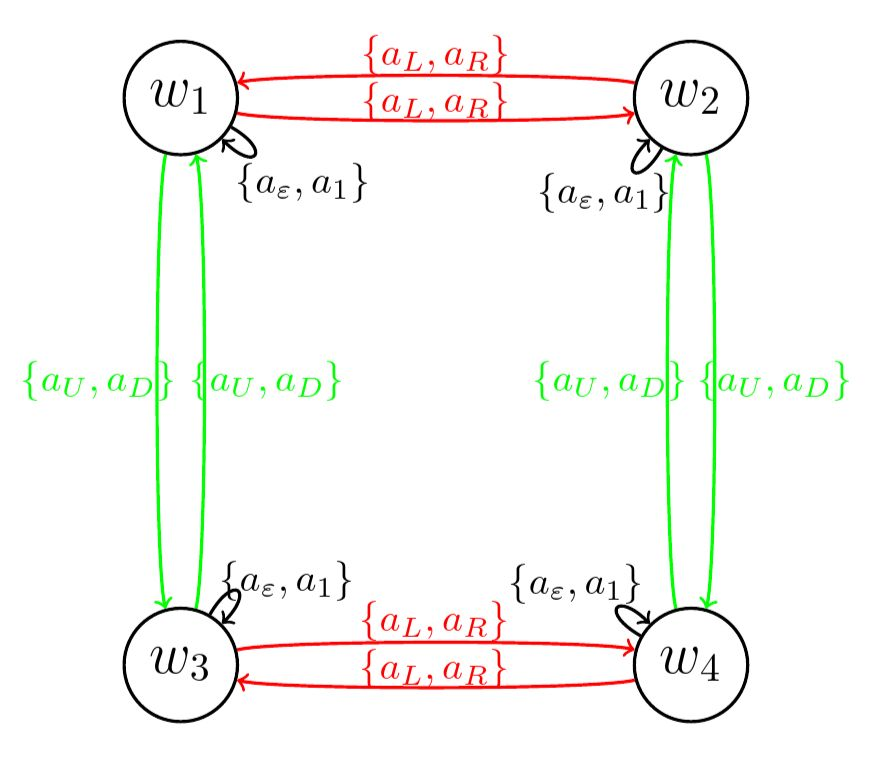
\includegraphics[width=0.5\linewidth]{2MathematicalFramework/Images/2x2_cyclical_equivalence_min_actions.jpeg}
	\caption{World diagram showing the minimum action equivalence classes under $\sim$ for the set $\hat{A} \cup \varepsilon$.}
	\label{fig:2x2_cyclical_equivalence_min_actions}
\end{figure}

\draftnote{blue}{awjdean}{
	Show diagrams with some non-minimum action transformations.
	Make it clear that equivalence classes contain more elements: $\{\varepsilon, 1 \dots \}$.
}

\draftnote{blue}{awjdean}{
	Map showing actions being sent to their equivalence classes under $\sim$: $D_{A}$ -($l$)-> $\hat{A}^{\ast}$ -($\pi_{A}$)-> $\hat{A}^{\ast}/\sim$.
}

%%%%%%%%%%%%%%%%%%%%%%%%%%%%%%%%%%%%%%%%%%%%%%%
\draftnote{red}{DIVIDER}{}
\draftnote{green}{To do}{
	\begin{enumerate}
		\item Equivalence relation $\sim$ for transformations and how it compares to equivalence relation $\sim$ for actions.
		\item \textbf{Mention:} Our use of an equivalence relation was inspired by \cite{caselles2020sensory}, which uses a similar equivalence relation to equate action sequences that cause the same final observation state after each action sequence is performed from an initial observation state.
	\end{enumerate}
}
\draftnote{red}{DIVIDER}{}
